%%%%%%%%%%%%%%%%%%%%%%%%%%%%%%
%
% $Autor: Wings $
% $Datum: 2019-12-09 11:50:02Z $
% $Pfad: komponenten/Bilderkennung/Produktspezifikation/CorelTPU/TPU/Allgemein/tikzdefs.tex $
% $Version: 1766 $
%
%
%%%%%%%%%%%%%%%%%%%%%%%%%%%%%%


% Definition für tikz

\usepackage{pgfplots}
\usepackage{pgf,tikz}
\usepackage{mathrsfs}
\usepackage{circuitikz}
\usepackage{tikz}
\usetikzlibrary{shapes,shapes.symbols,shapes.misc, shapes.multipart, shapes.geometric,arrows,angles,quotes,babel,positioning,calc,math,matrix,backgrounds}
\usetikzlibrary{positioning,fadings,through}


\usepackage{tikz-3dplot}

\definecolor{ArduinoColor}{rgb}{0.1,0.5,0.6}
\definecolor{BlackGreen}{rgb}{0.5, 0.68,0.375}
\definecolor{Or}{rgb}{0.945, 0.768,0.0588}
\definecolor{Cyann}{rgb}{0.1,0.9,0.9}


\tikzset{
  input2/.style={ % requires library shapes.geometric
    draw,
    trapezium,
    trapezium left angle=60,
    trapezium right angle=120,
  },
  process rectangle outer width/.initial=0.15cm,
  predefined process/.style={
    rectangle,
    draw,
    append after command={
      \pgfextra{
        \draw [fill=blue!20]
        ($(\tikzlastnode.north west)-(0,0.5\pgflinewidth)$)--
        ($(\tikzlastnode.north west)-(\pgfkeysvalueof{/tikz/process rectangle outer width},0.5\pgflinewidth)$)--
        ($(\tikzlastnode.south west)+(-\pgfkeysvalueof{/tikz/process rectangle outer width},+0.5\pgflinewidth)$)--
        ($(\tikzlastnode.south west)+(0,0.5\pgflinewidth)$);
        \draw [fill=blue!20]
        ($(\tikzlastnode.north east)-(0,0.5\pgflinewidth)$)--
        ($(\tikzlastnode.north east)+(\pgfkeysvalueof{/tikz/process rectangle outer width},-0.5\pgflinewidth)$)--
        ($(\tikzlastnode.south east)+(\pgfkeysvalueof{/tikz/process rectangle outer width},0.5\pgflinewidth)$)--
        ($(\tikzlastnode.south east)+(0,0.5\pgflinewidth)$);
      }  
    },
    text width=#1,
    align=center, fill=blue!20,  minimum height=4em
  },
  predefined process/.default=20mm,
  data1/.style={
    trapezium, 
    trapezium left angle=70, 
    trapezium right angle=110, 
    text width=1.5cm, 
    inner ysep=17pt,
    align=center, 
    line width=2pt,
    fill=blue!20
  },      
}


%Kabinettprojektion von 3D auf 2D
%
% Eingabe
% x,y,z
%
% Ausgabe
% x- oder y-Wert des Punkts
\newcommand{\Proj}[3]{({#1-#3*0.5*cos(30)},{#2-#3*0.5*sin(30)})}
\tikzset{declare function={ProjX(\x,\y,\z)=\x-\z*0.5*cos(30);}}
\tikzset{declare function={ProjY(\x,\y,\z)=\y-\z*0.5*sin(30);}}

%Rotation um die x-Achse 
%
% Eingabe
% x,y,z,alpha
%
% Ausgabe
% 
% x-, y- oder z-Wert des Punkts
\tikzset{declare function={RotXx(\x,\y,\z,\a)=\x;}}
\tikzset{declare function={RotXy(\x,\y,\z,\a)=\y*cos(\a)-\z*sin(\a);}}
\tikzset{declare function={RotXz(\x,\y,\z,\a)=\y*sin(\a)+\z*cos(\a);}}


%Rotation um die y-Achse 
%
% Eingabe
% x,y,z,alpha
%
% Ausgabe
% 
% x-, y- oder z-Wert des Punkts
\tikzset{declare function={RotYx(\x,\y,\z,\a)=\x*cos(\a)-\z*sin(\a);}}
\tikzset{declare function={RotYy(\x,\y,\z,\a)=\y;}}
\tikzset{declare function={RotYz(\x,\y,\z,\a)=\x*sin(\a)+\z*cos(\a);}}



%Rotation um die z-Achse 
%
% Eingabe
% x,y,z,alpha
%
% Ausgabe
% 
% x-, y- oder z-Wert des Punkts
\tikzset{declare function={RotZx(\x,\y,\z,\a)=\x*cos(\a)-\y*sin(\a);}}
\tikzset{declare function={RotZy(\x,\y,\z,\a)=\x*sin(\a)+\y*cos(\a);}}
\tikzset{declare function={RotZz(\x,\y,\z,\a)=\z;}}


%Rotation um die x-Achse 
%
% Eingabe
% x,y,z,alpha
%
% Ausgabe
% Punkt {x}{y}{z}
\newcommand{\RotXx}[4]{#1}%
\newcommand{\RotXy}[4]{(cos(#4)*#2-sin(#4)*#3)}
\newcommand{\RotXz}[4]{(sin(#4)*#2+cos(#4)*#3)}%


\tikzset{declare function={bellshape(\x,\mu,\sigma)=exp(-(\x-\mu)^2/(2*\sigma^2));}}


%Rotation um die x-Achse mit Projektion
%
% Eingabe
% x,y,z,alpha
%
% Ausgabe
% Punkt ({x}, {y})
\newcommand{\RotXP}[4]%
{(%
{#1-(sin(#4)*#2+cos(#4)*#3)*0.5*cos(30)},%
{cos(#4)*#2-sin(#4)*#3-(sin(#4)*#2+cos(#4)*#3)*0.5*sin(30)})%
}

%Rotation um die y-Achse mit Projektion
%
% Eingabe
% x,y,z,alpha
%
% Ausgabe
% Punkt ({x}, {y})
\newcommand{\RotYP}[4]%
{(%
{cos(#4)*#1+sin(#4)*#3-(-sin(#4)*#1+cos(#4)*#3)*0.5*cos(30)},%
{#2-(-sin(#4)*#1+cos(#4)*#3)*0.5*sin(30)}%
)}


%Rotation um die z-Achse mit Projektion
%
% Eingabe
% x,y,z,alpha
%
% Ausgabe
% Punkt ({x}, {y})
\newcommand{\RotZP}[4]%
{({cos(#4)*#1-sin(#4)*#2-#3*0.5*cos(30)},{sin(#4)*#1+cos(#4)*#2-#3*0.5*sin(30)})}


% Parameter
% #1: Skalierung
% #2: Winkel; 0..179
\newcommand{\HermiteSymPSP}[2]{%
  \pgfmathsetmacro{\RADIUS}{6}
  
  \begin{scope}[scale=#1]
    
    % angle 
    \begin{scope}[shift={(\RADIUS,0cm)}]
      \draw[fill=green!30] (0,0) -- (180:0.25*\RADIUS) arc (180:#2:0.25*\RADIUS);
      \draw ({0.5*(180+#2)}:{0.175*\RADIUS}) node {$\beta$};
      \draw ({0.5*(#2)}:{0.175*\RADIUS}) node {$\alpha$}; %$\pi-\alpha$
    \end{scope}
    
    \coordinate[label=left:$P_0$]  (P0) at (0,0);
    \coordinate  (t0) at (0.25*\RADIUS,0);
    \coordinate[label=below:$S$]  (S) at (\RADIUS,0);
    \coordinate  (s0) at (1.3*\RADIUS,0);
    \coordinate[label=left:$P_1$] (P1) at ({\RADIUS+\RADIUS*cos(#2)},{\RADIUS*sin(#2)});
    
    \draw [black,line width=0.5pt,domain=0:#2,->] plot ({\RADIUS+0.25*\RADIUS*cos(\x)}, {0+0.25*\RADIUS*sin(\x)});
    
    \draw [line width=1.5pt] (P0) -- (S) --(P1);
    \draw [line width=0.2pt,dotted] (S) --(s0);
    \node (P00) at (P0) {$\bullet$};
    \node (P11) at (P1) {$\bullet$};
  \end{scope}
}


% Parameter
% #1: Skalierung
% #2: Winkel; 0..179
\newcommand{\HermiteSym}[2]{%
   \pgfmathsetmacro{\RADIUS}{6}
  
   \begin{scope}[scale=#1]

     % angle 
     \begin{scope}[shift={(\RADIUS,0cm)}]
       \draw[fill=green!30] (0,0) -- (180:0.25*\RADIUS) arc (180:#2:0.25*\RADIUS);
       \draw ({0.5*(180+#2)}:{0.175*\RADIUS}) node {$\beta$};
       \draw ({0.5*(#2)}:{0.175*\RADIUS}) node {$\alpha$}; %$\pi-\alpha$
     \end{scope}

     \coordinate[label=left:$P_0$]  (P0) at (0,0);
     \coordinate  (t0) at (0.25*\RADIUS,0);
     \coordinate[label=below:$S$]  (S) at (\RADIUS,0);
     \coordinate  (s0) at (1.3*\RADIUS,0);
     \coordinate[label=left:$P_1$] (P1) at ({\RADIUS+\RADIUS*cos(#2)},{\RADIUS*sin(#2)});
     \coordinate (t1) at ({\RADIUS+ 1.25*\RADIUS*cos(#2)},{1.25*\RADIUS*sin(#2)});
  
     \coordinate[label=below:$\vec{t}_0$](T0) at ($ (P0)!.5!(t0) $);
     \coordinate[label=right:$\vec{t}_1$](T1) at ($ (P1)!.5!(t1) $);

     \draw [black,line width=0.5pt,domain=0:#2,->] plot ({\RADIUS+0.25*\RADIUS*cos(\x)}, {0+0.25*\RADIUS*sin(\x)});

     \draw [line width=1.5pt] (P0) -- (S) --(P1);
     \draw [line width=2pt,->,color=red] (P0) -- (t0);
     \draw [line width=2pt,->,color=red] (P1) -- (t1);
     \draw [line width=0.2pt,dotted] (S) --(s0);
     \node (P00) at (P0) {$\bullet$};
     \node (P11) at (P1) {$\bullet$};
  \end{scope}
}


% Parameter
% #1: Skalierung
% #2: Winkel; 0..-179
\newcommand{\HermiteSymNeg}[2]{%
  \pgfmathsetmacro{\RADIUS}{6}
  
  \begin{scope}[scale=#1]
    
    % angle 
    \begin{scope}[shift={(\RADIUS,0cm)}]
      \draw[fill=green!30] (0,0) -- (-180:0.25*\RADIUS) arc (-180:#2:0.25*\RADIUS);
      \draw ({0.5*(-180+#2)}:{0.175*\RADIUS}) node {$\beta$};
      \draw ({0.5*(#2)}:{0.175*\RADIUS}) node {$\alpha$}; %$\pi-\alpha$
    \end{scope}
    
    \coordinate[label=left:$P_0$]  (P0) at (0,0);
    \coordinate  (t0) at (0.25*\RADIUS,0);
    \coordinate[label=above:$S$]  (S) at (\RADIUS,0);
    \coordinate  (s0) at (1.3*\RADIUS,0);
    \coordinate[label=left:$P_1$] (P1) at ({\RADIUS+\RADIUS*cos(#2)},{\RADIUS*sin(#2)});
    \coordinate (t1) at ({\RADIUS+ 1.25*\RADIUS*cos(#2)},{1.25*\RADIUS*sin(#2)});
    
    \coordinate[label=below:$\vec{t}_0$](T0) at ($ (P0)!.5!(t0) $);
    \coordinate[label=right:$\vec{t}_1$](T1) at ($ (P1)!.5!(t1) $);
    
    \draw [black,line width=0.5pt,domain=0:#2,->] plot ({\RADIUS+0.25*\RADIUS*cos(\x)}, {0+0.25*\RADIUS*sin(\x)});
    
    \draw [line width=1.5pt] (P0) -- (S) --(P1);
    \draw [line width=2pt,->,color=red] (P0) -- (t0);
    \draw [line width=2pt,->,color=red] (P1) -- (t1);
    \draw [line width=0.2pt,dotted] (S) --(s0);
    \node (P00) at (P0) {$\bullet$};
    \node (P11) at (P1) {$\bullet$};
  \end{scope}
}

\tikzstyle{bigblock} = [draw, fill=blue!20, rectangle, minimum height=1.5em, minimum width=8em]
\tikzstyle{mediumblock} = [draw, fill=red!20, rectangle, minimum height=1.5em, minimum width=4em]
\tikzstyle{smallblock} = [draw, fill=red!20, rectangle, minimum height=1.5em, minimum width=1.5em]
\tikzstyle{arrow} = [->,shorten >=1pt,>=stealth',semithick]

\definecolor{LightCyan}{rgb}{0.88,1,1}
\definecolor{frenchblue}{rgb}{0.0, 0.45, 0.73}
\definecolor{greenblue}{rgb}{0.0, 0.25, 0.3}
\definecolor{darkcyan}{rgb}{0.0, 0.55, 0.55}
\definecolor{bondiblue}{rgb}{0.0, 0.58, 0.71}
\definecolor{grayleft}{rgb}{0.1, 0.1, 0.1}
\definecolor{grayright}{rgb}{0.2, 0.2, 0.2}
\definecolor{graycircle}{rgb}{0.3, 0.3, 0.3}
\definecolor{graylight}{rgb}{0.8, 0.8, 0.8}
\definecolor{greenenglish}{rgb}{0.0, 0.5, 0.0}
\definecolor{darkpastelgreen}{rgb}{0.01, 0.75, 0.24}
\definecolor{copper}{rgb}{0.72, 0.45, 0.2}
\definecolor{greenyellow}{rgb}{0.68, 1.0, 0.18}
\definecolor{fuchsia}{rgb}{1.0, 0.0, 1.0}
\definecolor{silver}{rgb}{0.75, 0.75, 0.75}
\definecolor{deepskyblue}{rgb}{0.0, 0.75, 1.0}

% Beispiele
%
%\begin{center}
%  \begin{tikzpicture}
%  \HermiteSym{1}{120}
%  \end{tikzpicture}
%\end{center}
%
%\begin{center}
%  \begin{tikzpicture}
%  \HermiteSym{1}{70}
%  \end{tikzpicture}
%\end{center}
%
%\begin{center}
%  \begin{tikzpicture}
%  \HermiteSym{1}{20}
%  \end{tikzpicture}
%\end{center}
%
%\begin{center}
%  \begin{tikzpicture}
%  \HermiteSym{1}{0}
%  \end{tikzpicture}
%\end{center}
%
%
%\begin{center}
%  \begin{tikzpicture}
%  \HermiteSymNeg{1}{-20}
%  \end{tikzpicture}
%\end{center}
%
%\begin{center}
%  \begin{tikzpicture}
%  \HermiteSymNeg{1}{-70}
%  \end{tikzpicture}
%\end{center}
%
%
%\begin{center}
%  \begin{tikzpicture}
%  \HermiteSymNeg{1}{-120}
%  \end{tikzpicture}
%\end{center}
%

%tikz-Kommandos

% Basis eines Roboters
% #1: Drehung des Systems
% #2: X-Offset des gedrehten Systems
% #3: Y-Offset des gedrehten Systems
% #4: Skalierung
\newcommand{\BASE}[4]{
  \begin{scope}[rotate=#1,scale=#4]  
    
    \draw[ultra thick, black]   ({#2-0.5},{#3-0.7}) -- ({#2+0.5},{#3-0.7});
    \draw[ultra thick, black]   ({#2-0.3},{#3-0.7}) -- ({#2-0.5},{#3-0.9});    
    \draw[ultra thick, black]   ({#2-0.1},{#3-0.7}) -- ({#2-0.3},{#3-0.9});    
    \draw[ultra thick, black]   ({#2+0.1},{#3-0.7}) -- ({#2-0.1},{#3-0.9});    
    \draw[ultra thick, black]   ({#2+0.3},{#3-0.7}) -- ({#2+0.1},{#3-0.9});    
    \draw[ultra thick, black]   ({#2+0.5},{#3-0.7}) -- ({#2+0.3},{#3-0.9});    
    
    \draw[thick, fill=blue!20]   ({#2-0.25},{#3-0.7}) -- ({#2+0.25},{#3-0.7}) -- ({#2},{#3}) -- ({#2-0.25},{#3-0.7});
    \draw[black, thick, fill=black]  (#2,#3) ellipse (0.1 and 0.1);
  \end{scope}
}%  


% Drehgelenk eines Roboters
% #1: Drehung des Gelenks
% #2: X-Offset des Systems
% #3: Y-Offset des Systems
% #4: Skalierung
\newcommand{\LINK}[4]{
  \begin{scope}[scale=#4]
    \draw[green, thick, fill=green!20]  ({#2+0.0},{#3+0.0}) ellipse (0.2 and 0.2);
    \draw[green, thick, fill=green!20]  ({#2+2.0*cos(#1)},{#3+2.0*sin(#1)}) ellipse (0.2 and 0.2);
    \draw[green!20, thick, fill=green!20]
    ({#2+0+0.2*cos(90+#1)},{#3+0+0.2*sin(90+#1)})
    --
    ({#2+2.0*cos(#1)+0.2*cos(90+#1)},{#3+2.0*sin(#1)+0.2*sin(90+#1)})
    --
    ({#2+2.0*cos(#1)+0.2*cos(-90+#1)},{#3+2.0*sin(#1)+0.2*sin(-90+#1)})
    --
    ({#2+0+0.2*cos(-90+#1)},{#3+0+0.2*sin(-90+#1)})
    --
    ({#2+0+0.2*cos(90+#1)},{#3+0+0.2*sin(90+#1)});
    \draw[green, thick]
    ({#2+0+0.2*cos(90+#1)},{#3+0+0.2*sin(90+#1)})
    --
    ({#2+2.0*cos(#1)+0.2*cos(90+#1)},{#3+2.0*sin(#1)+0.2*sin(90+#1)});
    \draw[green, thick]
    ({#2+2.0*cos(#1)+0.2*cos(-90+#1)},{#3+2.0*sin(#1)+0.2*sin(-90+#1)})
    --
    ({#2+0+0.2*cos(-90+#1)},{#3+0+0.2*sin(-90+#1)});
    \draw[black, thick, fill=blue]  ({#2+0.0},{#3+0.0}) ellipse (0.1 and 0.1);
    \draw[black, thick, fill=black]  ({#2+2*cos(#1)},{#3+2*sin(#1)}) ellipse (0.1 and 0.1);
    
  \end{scope}
}%  

% Drehgelenk eines Roboters
% #1: 1.Punkt x
% #2: 1.Punkt y
% #3: 2.Punkt x
% #4: 2.Punkt y
\newcommand{\LINKP}[4]{
  \begin{scope}
     \tikzmath{
       \Px  = #1;
       \Py  = #2;
       \Qx  = #3;
       \Qy  = #4;
       \Dx   = \Qx-\Px;
       \Dy   = \Qy-\Py;
       \Winkel = 45;
       \Pp  = \Dy*pow(\Dx,-1);
       \Winkel = atan(\Pp);
       \Laenge = pow(pow(\Dx,2)+pow(\Dy,2),0.5);
     }    
    
  
    \LINK{\Winkel}{#1}{#2}{1}
  \end{scope}
}%  

% SCARA-Roboters
% #1: Drehung des Systems
% #2: X-Offset des gedrehten Systems
% #3: Y-Offset des gedrehten Systems
% #4: Winkel des 1.Gelenks
% #5: Winkel des 2.Gelenks
% #6: Skalierung
% #7: Auswahl ungerade mit Beschriftung der Armlängen 
%           2 und 3: mit Winkel

\newcommand{\SCARA}[7]{
  \def\Rot{#1}
  \def\OffsetX{#2}
  \def\OffsetY{#1}
  \def\Alpha{#4}
  \def\Beta{#5}
  \def\Auswahl{#7}
  
  \begin{scope}[scale=#6]
    \BASE{\Rot}{\OffsetX}{\OffsetY}{1}
    \LINK{\Alpha}{\OffsetX}{\OffsetY}{1}
    \LINK{\Beta}{\OffsetX+2*cos(\Alpha)}{\OffsetY+2*sin(\Alpha)}{1}
    
    \ifthenelse{\isodd{\Auswahl}}
    {
        \node (Q1T) at (\OffsetX-0.6,\OffsetY) {$(0,0)$};
        \node (Q2T) at ({\OffsetX+1*cos(\Alpha)-0.4*sin(\Alpha)},{\OffsetY+1*sin(\Alpha)+0.4*cos(\Alpha)}) {$\ell_1$};
        \node (Q3T) at ({\OffsetX+2*cos(\Alpha)+1*cos(\Alpha+\Beta)+0.2*sin(\Alpha+\Beta)},{\OffsetY+2*sin(\Alpha)+1*sin(\Alpha+\Beta)-     0.2*cos(\Alpha+\Beta)}) {$\ell_2$};
    }{}    
    
    \ifthenelse{\equal{\Auswahl}{2}\or \equal{\Auswahl}{3}}
    {    
      \draw[color=red] ({cos(\Rot)*\OffsetX+sin(\Rot)*\OffsetY},
                       {-sin(\Rot)*\OffsetX+cos(\Rot)*\OffsetY})
              --
                    ({cos(\Rot)*(\OffsetX+1)+sin(\Rot)*\OffsetY},
                    {-sin(\Rot)*(\OffsetX+1)+cos(\Rot)*\OffsetY});
      \draw[color=red]
         ({cos(\Rot+\Alpha)*\OffsetX-sin(\Rot+\Alpha)*\OffsetY},
          {sin(\Rot+\Alpha)*\OffsetX+cos(\Rot+\Alpha)*\OffsetY})
          --
       ({cos(\Rot-\Alpha)*(\OffsetX+1)-sin(\Rot-\Alpha)*\OffsetY},
       {sin(\Rot+\Alpha)*(\OffsetX+1)+cos(\Rot+\Alpha)*\OffsetY});

      \draw[color=red] ({cos(\Rot)*(\OffsetX+2*cos(\Alpha))
                           +sin(\Rot)*(\OffsetY+2*sin(\Alpha))},
                       {-sin(\Rot)*(\OffsetX+2*cos(\Alpha))+cos(\Rot)*(\OffsetY+2*sin(\Alpha))})
              --
                    ({cos(\Rot+\Alpha)*((\OffsetX+2*cos(\Alpha))+1)+sin(\Rot+\Alpha)*(\OffsetY+2*sin(\Alpha))},
                    {-sin(\Rot-\Alpha)*((\OffsetX+2*cos(\Alpha))+1)+cos(\Rot-\Alpha)*(\OffsetY+2*sin(\Alpha))});

      \draw[color=red] ({cos(\Rot)*(\OffsetX+2*cos(\Alpha))
                           +sin(\Rot)*(\OffsetY+2*sin(\Alpha))},
                       {-sin(\Rot)*(\OffsetX+2*cos(\Alpha))+cos(\Rot)*(\OffsetY+2*sin(\Alpha))})
              --
                    ({cos(\Rot+\Alpha+\Beta)*((\OffsetX+2*cos(\Alpha))+1)+sin(\Rot+\Alpha+\Beta)*(\OffsetY+2*sin(\Alpha))},
                    {-sin(\Rot-\Alpha+\Beta)*((\OffsetX+2*cos(\Alpha))+1)+cos(\Rot-\Alpha+\Beta)*(\OffsetY+2*sin(\Alpha))});

    }{}    
  \end{scope}
}%  


% Nicht fertig
\newcommand{\SCARAXY}[6]{
  \begin{scope}[scale=#6]
    \def\ScaraX{#1}
    \def\ScaraY{#2}
    %ang2=90-(ACOS((L1^2-L2^2+x^2+y^2)/(2*L1*RAIZ(x^2+y^2)))+(ATAN(x/y))
    \def\ScaraTheta2{3.1415926*0.5-acos((sqrt(\ScaraX^2+\ScaraY^2)/4)+atan(\ScaraX/\ScaraY)}
    %angB=180-ACOS((L1^2+L2^2-x^2-y^2)/(2*L1*L2))
    \def\AngleB{3.1415926-acos((8-\ScaraX^2-\ScaraY^2)/8}
    % ang1=ang2+angB
    \def\ScaraTheta2{\ScaraTheta2+\AngleB}
  \end{scope}
}%  

% Planarer Roboter mit 3 Links
% #1: Drehung des Systems
% #2: X-Offset des gedrehten Systems
% #3: Y-Offset des gedrehten Systems
% #4: Winkel des 1.Gelenks
% #5: Winkel des 2.Gelenks
% #6: Winkel des 3.Gelenks
% #6: Skalierung

\newcommand{\RRRPLANAR}[7]{
  \def\Rot{#1}
  \def\OffsetX{#2}
  \def\OffsetY{#1}
  \def\Alpha{#4}
  \def\Beta{#5}
  \def\Gamma{#6}
  
  \begin{scope}[scale=#7]
    \BASE{\Rot}{\OffsetX}{\OffsetY}{1}
    \LINK{\Alpha}{\OffsetX}{\OffsetY}{1}
    \LINK{\Beta}{\OffsetX+2*cos(\Alpha)}{\OffsetY+2*sin(\Alpha)}{1}
    \LINK{\Gamma}{\OffsetX+2*cos(\Alpha)+2*cos(\Beta)}{\OffsetY+2*sin(\Alpha)+2*sin(\Beta)}{1}
  \end{scope}
}%  
    


% Kreisbogen
%\draw [green,line width=0.5pt,domain=0:180] plot ({5+1*cos(\x)}, {3+1*sin(\x)});


\newcommand{\tstar}[5]{% inner radius, outer radius, tips, rot angle, options
  \pgfmathsetmacro{\starangle}{360/#3}
  \draw[#5] (#4:#1)
  \foreach \x in {1,...,#3}
  { -- (#4+\x*\starangle-\starangle/2:#2) -- (#4+\x*\starangle:#1)
  }
  -- cycle;
}


\newcommand{\ngram}[4]{% outer radius, tips, rot angle, options
  \pgfmathsetmacro{\starangle}{360/#2}
  \pgfmathsetmacro{\innerradius}{#1*sin(90-\starangle)/sin(90+\starangle/2)}
  \tstar{\innerradius}{#1}{#2}{#3}{#4}
}


% Zeichnen der Scherenkinematik
% Die ersten Parameter sind X und Y-Position
% Der dritte Parameter zeigt gegebenenfalls Bezeichnungen:
% 0 : Keine Bezeichnung
% 1 : Veränderliche Parameter
% 2 : Konstrukvie Parameter
% 3 : Alle Parameter
\newcommand{\Scissor}[3]%
{
  \begin{center}
    \begin{tikzpicture}
      \def\ScissorX{#1}
      \def\ScissorY{#2}
      \def\Auswahl{#3}
    
      \tikzmath{\HF  =  8; % Rahmenhoehe
                \DF  = 12.5; % Rahmenbreite
                \BF  = 0.2; % Breite der Balken
                \Arm = 6;   % Länge des Arms
                \DS  = 0.6; % Breite der Zange
                \HS  = 0.3; % Höhe der Zange
                \PLx = \ScissorX-0.5*\DS;
                \PRx = \ScissorX+0.5*\DS;
                \Py  = \HF-\ScissorY+\HS;                
                \QL  = \PLx-pow(\Arm*\Arm-pow(\ScissorY-\HS,2),0.5); 
                \QR  = \PRx+pow(\Arm*\Arm-pow(\ScissorY-\HS,2),0.5);
               }
%               
      \draw[thick=4pt,fill] 
              (-\BF,0) -- (0,0) -- (0,\HF) -- (\DF,\HF) -- (\DF,0) -- (\DF+\BF,0) 
              -- (\DF+\BF,\HF+\BF) -- (-\BF,\HF+\BF) -- (-\BF,0);
      
      \draw[thick=2pt,red] 
         (\QL,{\HF+0.5*\BF}) -- (\PLx,\Py) -- (\PRx, \Py) -- (\QR,{\HF+0.5*\BF});
      \draw[thick=2pt,red,fill] 
            (\PLx,\Py) -- (\PRx, \Py) -- ({\ScissorX},{\HF-\ScissorY}) -- (\PLx,\Py);
       
      \draw [green,thick,domain=0:360,fill] plot ({\QL+0.5*\BF*cos(\x)}, {\HF+0.5*\BF+0.5*\BF*sin(\x)});
      \draw [green,thick,domain=0:360,fill] plot ({\QR+0.5*\BF*cos(\x)}, {\HF+0.5*\BF+0.5*\BF*sin(\x)});
      
      
      \draw [green,thick,domain=0:360,fill] plot ({\ScissorX+0.5*\BF*cos(\x)}, {\HF-\ScissorY+0.5*\BF+0.5*\BF*sin(\x)});
     
      \draw [green,thick,domain=0:360,fill] 
         plot (
                {\PLx+0.5*\BF*cos(\x)}, 
                {\Py+0.5*\BF*sin(\x)}
              );
      \draw [green,thick,domain=0:360,fill] 
        plot (
          {\PRx+0.5*\BF*cos(\x)}, 
          {\Py+0.5*\BF*sin(\x)}
        );
        
%        \LINK{-45}{\QL}{\HF}{1};

  \ifthenelse{\isodd{\Auswahl}}
  {
      \node (Q1T) at (\QL,\HF+\BF+0.3) {$q_l$};
      \node (Q2T) at (\QR,\HF+\BF+0.3) {$q_r$};
%      
  %Beschriftung
      \node (PL) at (\PLx-0.3,\Py) {$P_l$};
      \node (PR) at (\PRx+0.3,\Py) {$P_r$};
      \node (TCP) at (\ScissorX,\Py-0.3-\HS) {$(X,Y)$};
  }{}    
      
  \ifthenelse{\equal{\Auswahl}{2}\or \equal{\Auswahl}{3}}
  {
    % Konstruktive Parameter
      \draw (-\BF-0.3,0)  -- (-\BF-0.6,0);
      \draw (-\BF-0.3,\HF)  -- (-\BF-0.6,\HF);
      \draw[->]  ({-\BF-0.45},{\HF*0.5-0.3}) -- ({-\BF-0.45},0);
      \draw[->] ({-\BF-0.45},{\HF*0.5+0.3}) -- ({-\BF-0.45},{\HF}) ;
      \node (HF) at ({-\BF-0.45},{\HF*0.5+0.3}) {$\HFrame$};

      \draw[<-] (-\BF,\HF+\BF+0.6)  -- (0.5*\DF-0.3,\HF+\BF+0.6);      
      \draw[->] (0.5*\DF+0.3,\HF+\BF+0.6)  -- (\DF,\HF+\BF+0.6);      
      \node (DF) at (0.5*\DF,\HF+\BF+0.6)  {$\LFrame$};
 
      \draw [<->]  (\PLx-0.6,\Py)  -- (\PLx-0.6,{\Py-\HS});
      \node (HS) at  (\PLx-0.9,{\Py-0.5*\HS}) {$\HTongs$};

      \draw [<->]  (\PLx,\Py+0.3)  -- (\PRx,{\Py+0.3});
      \node (DS) at  (\ScissorX,{\Py+0.6}) {$\LTongs$};
 
     \draw[<->] (\QL -0.6,{\HF+0.5*\BF-0.6}) -- (\PLx-0.6,\Py-0.6);
     \node (LArm) at ({0.5*(\QL +\PLx)-0.9},{0.5*(\HF+0.5*\BF+\Py)-0.6}  ) {$\LArm$};
 }{}       
    \end{tikzpicture}
  \end{center}
}


\newcommand{\ArduinoNanoBLESense}[4]%
{
  \def\LowerLeftX{#1}
  \def\LowerLeftY{#2}
  \def\UpperRightX{#3}
  \def\UpperRightY{#4}
    
  \node at (0,0) (Board) {\includegraphics{Arduino/Nano33BLE/Nano33BLESense}};

  \fill[gray, opacity=0.7] (-6,-2.4) rectangle (6,2.4);

  \coordinate (A) at (\LowerLeftX,\LowerLeftY);
  \coordinate (B) at (\UpperRightX,\UpperRightY);    
  \begin{scope}
    \clip (A) rectangle (B);
    
    \node at (0,0) (Board) {\includegraphics{Arduino/Nano33BLE/Nano33BLESense}};
    
  \end{scope}
  \draw[yellow,line width=2pt] (A)  rectangle (B);
}

\newcommand{\ArduinoNanoTikz}{
    \begin{scope}[scale=1.5,rotate=90]
        \fill[ArduinoColor] (0,0) rectangle (3,7);
        \fill[gray!45] (0.85,6.35) rectangle++ (1.3,1);
        \foreach \y in {6.45,6.65,6.85,7.05,7.25}{
            \fill[gray!30,gray!30] (0.85,\y) rectangle ++(1.3, 0.1); }
        \foreach \x in {1.2,1.33125,1.4625,1.59375,1.725}{
            \draw[fill=gray!15,gray!15] (\x, 6.23) rectangle++ (0.075, 0.12); }
        \foreach \y  in{0.5,0.9,1.3,1.7,2.1,2.5,2.9,3.3,3.7,4.1,4.5,4.9,5.3,5.7,6.1} {
            \fill[gray!30] (0,\y) rectangle ++(0.25, 0.26); 
            \fill[gray!30] (2.75,\y) rectangle ++(0.25,0.26);}
        \foreach \y in {0.63,1.03,1.43,1.83,2.23,2.63,3.03,3.43,3.83,4.23,4.63,5.03,5.43,5.83,6.23} {
            \fill[gray!30](0.25,\y) circle (0.13);
            \fill[gray!30](2.75,\y) circle (0.13);
            \draw[fill=gray!60,gray!60](0.25,\y) circle (0.11);
            \draw[fill=gray!60,gray!60](2.75,\y) circle (0.11);
            \fill[white,white](0,\y) circle (0.085);
            \fill[white,white](3,\y) circle (0.085); }		
        \foreach \x in {0.2, 2.8} {
            \draw[fill=white!100,white!100](\x,0.2) circle (0.12);}
        \draw[fill=gray!60,gray!60] (1.1,5.1) rectangle++ (0.8,0.2);
        \draw[fill=gray!30, gray!30] (1.2,5) rectangle++(0.6,0.4);				
        \draw[fill=white, white] (1.5,5.2) circle (0.16) ;
        \draw[fill=gray!60,gray!60] (0.70, 0.55) rectangle (2.3,2.1);
        \fill[gray!45] (0.75, 0.6) rectangle (2.25,2.05);
        \foreach \x in {0.5,2.35}{
            \draw[fill=gray!15,gray!15] (\x,6.5) rectangle ++(0.12, 0.3); }
        \foreach \x in {0.56,2.4}{
            \draw[fill=Or, Or] (\x,6.65) circle(0.1); }
        \foreach \x in {0.2,2.8}{
            \draw[fill=white, white] (\x,6.8) circle(0.15); }
        \draw[fill=BlackGreen, BlackGreen] (0.7, 0) rectangle(2.3,0.55); 
        \draw[fill=black!100](0.5,2.8) rectangle++ (0.35,0.35);		
        \draw[fill=black!100](1.65,4) rectangle++ (0.3, 0.3);		
        \draw[fill=black!100](0.5,5.25) rectangle++ (0.35,0.5);
        \foreach \y in {2.25, 2.41}{
            \draw[fill=Cyann!70, Cyann!70] (1.85, \y) rectangle++(0.11, 0.11);
            \draw[fill=Cyann!70, Cyann!70] (2.01, \y) rectangle++(0.11, 0.11); }
        \draw[fill=gray!60, gray!60] (1.9,2.3) rectangle++(0.17, 0.17);
        
        \foreach \x in {0.85, 1}{
            \draw[fill=gray!30,gray!30](\x, 3.25) rectangle++(0.08, 0.18);
            \draw[fill=gray!60,gray!60](\x, 3.265) rectangle++(0.08, 0.15);}
        \draw[fill=gray!30,gray!30](1.12, 2.9) rectangle++(0.08, 0.18);		
        \draw[fill=gray!60, gray!60](1.12, 2.915) rectangle++(0.08, 0.15);
        
        \draw[fill=black, black] (1.26, 2.25) rectangle (1.66, 2.85);	
        \fill[white, white] (1.45, 2.4) circle(0.08);
        \fill[Or, Or] (1.45, 2.4) circle(0.06);
        \fill[white,white] (1.45, 2.4) circle(0.04);
        
        \draw[fill=black] (1.34,2.89) rectangle (1.66, 3.14);
        \draw[fill=black] (1.34,3.18) rectangle (1.66, 3.62);		
        \fill[white] (1.515, 3.5) circle(0.08);
        \fill[Or!30] (1.515, 3.5) circle(0.06);
        \draw[fill = black] (1.8, 3.1) rectangle(2.25, 3.62);
        
        \draw[fill=black] (0.5, 4.1) rectangle++ (0.8, 0.5);
        \foreach \x in {0.5714, 0.6928,0.8142,0.9357,1.0571,1.1782}{
            \draw[fill=gray!15,gray!15] (\x,4.05) rectangle++(0.05, 0.05);
            \draw[fill=gray!15,gray!15] (\x,4.6) rectangle++(0.05, 0.05);}
        \foreach \y in {4.16,4.27,4.38,4.49}{
            \draw[fill=gray!15,gray!15] (1.3,\y) rectangle++(0.05, 0.05); }
        \draw[fill=black] (1.6,5.6) rectangle++(0.25, 0.35); 
        \foreach \y in {5.65, 5.86}{
            \draw[fill=gray!45,gray!45] (1.47,\y) rectangle++(0.16, 0.04); 
            \draw[fill=gray!45,gray!45] (1.82,\y) rectangle++(0.16, 0.04);}
        
        \draw[fill=black] (2.05,5.5) rectangle++(0.24, 0.4); 
        \draw[fill=gray!30,gray!30] (2.15, 5.4) rectangle++(0.04, 0.15); 
        \draw[fill=gray!30,gray!30] (2.15,5.85) rectangle++(0.04, 0.15);
        
        \draw[rounded corners=2pt, fill=black] (1.15,5.6) rectangle++ (0.2,0.3);
        \foreach \y in {5.55, 5.85}{
            \fill[gray!45, opacity=0.7] (1.12,\y) rectangle++ (0.26, 0.1);}		
        \draw[rounded corners=2pt, fill=black] (2.1,4.4) rectangle++ (0.2,0.3);
        \foreach \y in {4.35, 4.65}{
            \fill[gray!45, opacity=0.8] (2.08,\y) rectangle++ (0.24, 0.1);}
        \foreach \y  in {4.35, 4.55}{
            \fill[gray!30,gray!30](1.7, \y) rectangle++ (0.22, 0.1);
            \fill[gray!60,gray!60](1.71, \y) rectangle++ (0.20, 0.1);}
        \draw[rounded corners=2pt, fill=black] (0.9,3.75) rectangle++ (0.3,0.2);
        \foreach \x in {0.85, 1.15}{
            \fill[gray!45, opacity=0.8] (\x,3.72) rectangle++ (0.1, 0.26);}		
        \foreach \y  in {2.6, 3.2, 3.4}{
            \draw[rounded corners=1pt, fill=gray!30,gray!30](0.5,\y) rectangle++ (0.2, 0.1); }
        \foreach \y  in {2.6, 3.2, 3.4}{		
            \draw [fill=gray!60,gray!60] (0.55, \y ) rectangle++ (0.1, 0.1); }
        
        \draw[rounded corners=1pt, fill=gray!30,gray!30](2.45,0.9) rectangle++ (0.1, 0.2);
        \draw [fill=gray!60, gray!60] (2.45, 0.95 ) rectangle++ (0.1, 0.1);
        
        \foreach \y in {0.2, 0.5}{
            \draw[rounded corners=1pt, fill=gray!30,gray!30] (0.5,\y) rectangle++ (0.1,0.2);}
        \foreach \y in {0.25, 0.55}{
            \draw [fill=gray!60,gray!60] (0.5, \y) rectangle++ (0.1, 0.1);}
        \draw [fill=gray!30,gray!30] (0.5, 1.7) rectangle++ (0.1, 0.2);
        \draw [fill=gray!60,gray!60] (0.5, 1.72) rectangle++ (0.1, 0.16);
        \foreach \x in {1.7, 2.2}{
            \draw[rounded corners=1pt, fill=gray!30,gray!30] (\x, 2.25 ) rectangle++ (0.1,0.2);}
        \foreach \x in {1.7, 2.2}{
            \draw [fill=gray!60,gray!60] (\x,2.3) rectangle++ (0.1, 0.1);}
        \draw[rounded corners=1pt, fill=gray!30, gray!30](2,2.7) rectangle++ (0.2,0.1);
        \draw [fill=gray!60,gray!60] (2.05,2.7) rectangle++ (0.1, 0.1);
        \foreach \x in {2, 2.2}{
            \draw[rounded corners=1pt, fill=gray!30,gray!30] (\x,5.1) rectangle++ (0.1,0.2);}
        \foreach \x in {2, 2.2}{
            \draw [fill=gray!60,gray!60] (\x,5.15) rectangle++ (0.1, 0.1);}
        
        \draw[rounded corners=1pt, fill=gray!30,gray!30] (0.6,6.0) rectangle++ (0.1,0.2);
        \draw [fill=gray!60,gray!60] (0.6,6.05) rectangle++ (0.1, 0.1);
        \draw[rounded corners=1pt, fill=gray!30,gray!30] (0.95,5.5) rectangle++ (0.1,0.2);
        \draw [fill=gray!60,gray!60] (0.95,5.55) rectangle++ (0.1, 0.1);
        \draw [fill=gray!30,gray!30] (0.7,5.85) rectangle++ (0.2, 0.1);
        \draw [fill=gray!60,gray!60] (0.72,5.85) rectangle++ (0.16, 0.1);
        
        \draw[rounded corners=1pt, fill=gray!30,gray!30] (2.5,6.2) rectangle++ (0.1,0.2);
        \draw [fill=gray!60,gray!60] (2.5,6.25) rectangle++ (0.1, 0.1);
        \draw[rounded corners=1pt, fill=gray!30,gray!30] (2.3,3.85) rectangle++ (0.1,0.2);
        \draw [fill=gray!60,gray!60] (2.3,3.9) rectangle++ (0.1, 0.1);
        \draw[rounded corners=1pt, fill=gray!30, gray!30] (2.15,4) rectangle++ (0.1,0.2);
        \draw [fill=gray!60,gray!60] (2.15,4.05) rectangle++ (0.1, 0.1);		
        
        \draw[rounded corners=1pt, fill=gray!30, gray!30](1.4,3.75)  rectangle++ (0.2,0.1);
        
        \draw [fill=gray!60,gray!60] (1.45,3.75) rectangle++ (0.1, 0.1);
        
        \draw[rounded corners=1pt, fill=gray!30, gray!30](1.45,4)  rectangle++ (0.1,0.2);
        \draw [fill=gray!60,gray!60] (1.45,4.05) rectangle++ (0.1, 0.1);
        \foreach \y  in {3.1, 3.5}{
            \draw[rounded corners=1pt, fill=gray!30, gray!30](2.5,\y) rectangle++ (0.1, 0.2); }
        \foreach \y  in {3.15,3.55}{		
            \draw [fill=gray!60,gray!60] (2.5, \y ) rectangle++ (0.1, 0.1); }
        
        
        \draw[rounded corners=1pt, fill=gray!30, gray!30](0.65,4.9)  rectangle++ (0.2,0.1);
        \draw [fill=gray!60,gray!60] (0.7,4.9) rectangle++ (0.1, 0.1);
        \draw [fill=gray!60,gray!60] (0.65,4.75) rectangle++ (0.2, 0.1);
        \draw [fill=gray!60,gray!60] (0.67,4.75) rectangle++ (0.16, 0.1);
        
        
        \draw[fill= ArduinoColor, ArduinoColor] (0.75,0.42) -- (2.25,0.42) -- (1.5,-0.2) -- cycle;
        \draw[fill=BlackGreen,BlackGreen] (0.7,0.48) rectangle++(0.1, -0.3);
        \draw[fill=BlackGreen, BlackGreen] (2.2,0.48) rectangle++(0.1, -0.3);
        \draw[fill=BlackGreen, BlackGreen] (0.9,0.15) rectangle++(1.1, 0.075);
        \draw[fill=BlackGreen, BlackGreen] (0.9,0) rectangle++(1.1, 0.05);
        \fill[white] (0,0) rectangle++(3, -2);
        
        \node[text= white, anchor=center] at (2.5,4.9) {\tiny{NANO 33 BLE SEENSE LITE}};
        
        \node[text= white, anchor=center] at (2.5,1.8) {\tiny{ARDUINO CC}};
        
%        \node at (-3,3.7) (Board) {\includegraphics[angle = 90]{Nano33BLESense}};	
    \end{scope}    
}    

\newcommand{\ArduinoNanoShieldTikz}{
  \fill[ArduinoColor] (0.29, 29.47) rectangle (11.06, 23.44);

  %linksoben der Knopf
  \fill[darkgray] (0.33, 28.68) rectangle (1.98, 27.2);
  \fill[lightgray] (0.45, 28.57) rectangle (1.84, 27.35);
  \fill[gray] (1.14, 27.96) ellipse (0.48cm and 0.45cm);
  \fill[black] (0.93, 28.15) rectangle (1.35, 27.78);

  %steckplatz Kamera
  \fill[darkgray] (6.71, 28.04) rectangle (7.35, 24.91);
  \fill[black] (6.76, 25.15) rectangle (6.96, 24.94);
  \fill[black] (7.1, 25.14) rectangle (7.29, 24.94);
  \fill[black] (6.76, 27.97) rectangle (6.95, 27.76);
  \fill[black] (7.09, 27.96) rectangle (7.29, 27.76);
  \fill[black] (6.76, 27.64) rectangle (6.95, 27.44);
  \fill[black] (7.1, 27.63) rectangle (7.29, 27.44);
  \fill[black] (6.77, 27.33) rectangle (6.96, 27.13);
  \fill[black] (7.1, 27.32) rectangle (7.29, 27.13);
  \fill[black] (6.76, 27.02) rectangle (6.96, 26.82);
  \fill[black] (7.1, 27.01) rectangle (7.29, 26.82);
  \fill[black] (6.77, 26.7) rectangle (6.96, 26.5);
  \fill[black] (7.1, 26.7) rectangle (7.29, 26.5);
  \fill[black] (6.77, 26.39) rectangle (6.96, 26.19);
  \fill[black] (7.11, 26.38) rectangle (7.3, 26.19);
  \fill[black] (6.76, 26.08) rectangle (6.96, 25.87);
  \fill[black] (7.1, 26.07) rectangle (7.29, 25.87);
  \fill[black] (6.76, 25.77) rectangle (6.95, 25.57);
  \fill[black] (7.1, 25.76) rectangle (7.29, 25.57);
  \fill[black] (6.76, 25.46) rectangle (6.95, 25.26);
  \fill[black] (7.1, 25.45) rectangle (7.29, 25.26);

  %Schraubenlöcher
  \fill[white] (10.72, 23.76) ellipse (0.25cm and 0.22cm);
  \fill[white] (10.68, 29.18) ellipse (0.25cm and 0.22cm);
  \fill[white] (0.65, 29.17) ellipse (0.25cm and 0.22cm);
  \fill[white] (0.64, 23.75) ellipse (0.25cm and 0.22cm);

  %Stromzufuhr
  \fill[green] (0.3, 25.34) rectangle (1.49, 24.0);
  \fill[black] (0.81, 24.97) ellipse (0.25cm and 0.23cm);
  \fill[black] (0.81, 24.36) ellipse (0.25cm and 0.23cm);
  \fill[darkgray] (0.7, 24.57) rectangle (0.92, 24.14);
  \fill[darkgray] (0.7, 25.18) rectangle (0.91, 24.75);
  \fill[white] (1.49, 25.12) rectangle (2.15, 24.89);
  \node[teal, font=\tiny] at (1.8,25) {GND};
  \node[white, font=\tiny] at (1.8,24.34) {VIN};

  %Arduino Steckplatz links
  \fill[darkgray] (2.35, 28.82) rectangle (2.71, 24.12);
  \fill[black] (2.41, 26.89) rectangle (2.63, 26.67);
  \fill[black] (2.41, 26.58) rectangle (2.63, 26.36);
  \fill[black] (2.41, 26.26) rectangle (2.63, 26.04);
  \fill[black] (2.41, 25.94) rectangle (2.63, 25.72);
  \fill[black] (2.41, 25.63) rectangle (2.63, 25.41);
  \fill[black] (2.41, 25.33) rectangle (2.63, 25.11);
  \fill[black] (2.41, 25.02) rectangle (2.63, 24.8);
  \fill[black] (2.41, 24.7) rectangle (2.63, 24.48);
  \fill[black] (2.41, 24.38) rectangle (2.63, 24.16);
  \fill[black] (2.4, 27.19) rectangle (2.63, 26.97);
  \fill[black] (2.41, 27.5) rectangle (2.64, 27.28);
  \fill[black] (2.42, 28.11) rectangle (2.65, 27.89);
  \fill[black] (2.42, 27.82) rectangle (2.65, 27.6);
  \fill[black] (2.42, 28.43) rectangle (2.64, 28.21);
  \fill[black] (2.43, 28.74) rectangle (2.65, 28.52);
  \fill[black] (2.48, 25.78) rectangle (2.5, 25.78);

  %Arduino Steckplatz rechts
  \fill[darkgray] (4.48, 28.82) rectangle (4.84, 24.12);
  \fill[black] (4.54, 26.89) rectangle (4.76, 26.67);
  \fill[black] (4.54, 26.58) rectangle (4.76, 26.36);
  \fill[black] (4.54, 26.26) rectangle (4.76, 26.04);
  \fill[black] (4.54, 25.94) rectangle (4.76, 25.72);
  \fill[black] (4.54, 25.62) rectangle (4.76, 25.41);
  \fill[black] (4.54, 25.33) rectangle (4.76, 25.11);
  \fill[black] (4.54, 25.02) rectangle (4.76, 24.8);
  \fill[black] (4.54, 24.7) rectangle (4.76, 24.48);
  \fill[black] (4.54, 24.38) rectangle (4.76, 24.16);
  \fill[black] (4.53, 27.19) rectangle (4.76, 26.97);
  \fill[black] (4.54, 27.5) rectangle (4.76, 27.28);
  \fill[black] (4.55, 28.11) rectangle (4.78, 27.89);
  \fill[black] (4.55, 27.81) rectangle (4.78, 27.6);
  \fill[black] (4.55, 28.43) rectangle (4.77, 28.21);
  \fill[black] (4.56, 28.74) rectangle (4.78, 28.52);
  \fill[black] (4.61, 25.78) rectangle (4.63, 25.78);
  \fill[black] (4.61, 25.78) rectangle (4.63, 25.78);

  %USB Seite vom Steckplatz mit weißer Umrandung
  \draw [ultra thick, white] (2.34,29.03) rectangle (4.85,23.81);
  \fill [teal] (3.1,29.23) rectangle (4.1,28);
  \draw [ultra thick, white] (3.1,29.23) rectangle (4.1,28);
  \node [rotate=270,white,font=\tiny] at (3.6,28.6) {USB};

  %Groove 6
  \fill[white] (9.9, 24.84) rectangle (10.15, 24.1);
  \fill[brown!20] (9.0, 24.15) rectangle (10.39, 23.43);
  \fill[brown!40] (9.56, 23.72) ellipse (0.12cm and 0.11cm);
  \fill[brown!40] (9.84, 23.72) ellipse (0.12cm and 0.11cm);
  \fill[brown!40] (10.12, 23.72) ellipse (0.12cm and 0.11cm);
  \fill[brown!40] (9.29, 23.72) ellipse (0.12cm and 0.11cm);
  \fill[brown!40] (9.29, 23.55) rectangle (10.11, 23.43);
  \node [rotate=270,teal,font=\tiny] at (10.025,24.52) {GND};
  \node [rotate=270,white,font=\tiny] at (9.725,24.52) {3V3};
  \node [rotate=270,white,font=\tiny] at (9.425,24.52) {SDA};
  \node [rotate=270,white,font=\tiny] at (9.125,24.52) {SCL};

  %Groove 5
  \fill[white] (7.89, 24.83) rectangle (8.14, 24.09);
  \fill[brown!20] (6.95, 24.1) rectangle (8.33, 23.43);
  \fill[brown!40] (7.51, 23.74) ellipse (0.12cm and 0.11cm);
  \fill[brown!40] (7.79, 23.74) ellipse (0.12cm and 0.11cm);
  \fill[brown!40] (8.07, 23.74) ellipse (0.12cm and 0.11cm);
  \fill[brown!40] (7.24, 23.74) ellipse (0.12cm and 0.11cm);
  \fill[brown!40] (7.24, 23.55) rectangle (8.06, 23.43);
  \node [rotate=270,teal,font=\tiny] at (8.01,24.52) {GND};
  \node [rotate=270,white,font=\tiny] at (7.71,24.52) {3V3};
  \node [rotate=270,white,font=\tiny] at (7.41,24.52) {SDA};
  \node [rotate=270,white,font=\tiny] at (7.11,24.52) {SCL};


  %Groove 4
  \fill[white] (5.89, 24.82) rectangle (6.14, 24.07);
  \fill[brown!20] (4.91, 24.11) rectangle (6.3, 23.43);
  \fill[brown!40] (5.47, 23.74) ellipse (0.12cm and 0.11cm);
  \fill[brown!40] (5.75, 23.74) ellipse (0.12cm and 0.11cm);
  \fill[brown!40] (6.03, 23.74) ellipse (0.12cm and 0.11cm);
  \fill[brown!40] (5.2, 23.75) ellipse (0.12cm and 0.11cm);
  \fill[brown!40] (5.2, 23.55) rectangle (6.02, 23.43);
  \node [rotate=270,teal,font=\tiny] at (6.01,24.52) {GND};
  \node [rotate=270,white,font=\tiny] at (5.71,24.52) {3V3};
  \node [rotate=270,white,font=\tiny] at (5.41,24.52) {SDA};
  \node [rotate=270,white,font=\tiny] at (5.11,24.52) {SDL};


  %Groove 3
  \fill[brown!20] (8.98, 29.49) rectangle (10.37, 28.84);
  \fill[brown!40] (9.54, 29.12) ellipse (0.12cm and 0.11cm);
  \fill[brown!40] (9.83, 29.12) ellipse (0.12cm and 0.11cm);
  \fill[brown!40] (10.1, 29.12) ellipse (0.12cm and 0.11cm);
  \fill[brown!40] (9.27, 29.13) ellipse (0.12cm and 0.11cm);
  \fill[brown!40] (9.27, 29.49) rectangle (10.1, 29.37);
  \fill[white] (9.1, 28.84) rectangle (9.35, 28.09);
  \node [rotate=270,teal,font=\tiny] at (9.225,28.455) {GND};
  \node [rotate=270,white,font=\tiny] at (9.525,28.455) {3V3};
  \node [rotate=270,white,font=\tiny] at (9.825,28.455) {A7};
  \node [rotate=270,white,font=\tiny] at (10.125,28.455) {A6};

  %Grove 2
  \fill[brown!20] (6.95, 29.47) rectangle (8.33, 28.82);
  \fill[brown!40] (7.51, 29.1) ellipse (0.12cm and 0.11cm);
  \fill[brown!40] (7.79, 29.1) ellipse (0.12cm and 0.11cm);
  \fill[brown!40] (8.07, 29.1) ellipse (0.12cm and 0.11cm);
  \fill[brown!40] (7.24, 29.11) ellipse (0.12cm and 0.11cm);
  \fill[brown!40] (7.24, 29.47) rectangle (8.06, 29.35);
  \fill[white] (7.08, 28.84) rectangle (7.33, 28.09);
  \node [rotate=270,teal,font=\tiny] at (7.205,28.455) {GND};
  \node [rotate=270,white,font=\tiny] at (7.505,28.455) {3V3};
  \node [rotate=270,white,font=\tiny] at (8.105,28.455) {D11};

  % Grove 1
  \fill[brown!20] (4.91, 29.49) rectangle (6.3, 28.84);
  \fill[brown!40] (5.47, 29.13) ellipse (0.12cm and 0.11cm);
  \fill[brown!40] (5.75, 29.13) ellipse (0.12cm and 0.11cm);
  \fill[brown!40] (6.03, 29.12) ellipse (0.12cm and 0.11cm);
  \fill[brown!40] (5.2, 29.13) ellipse (0.12cm and 0.11cm);
  \fill[brown!40] (5.2, 29.49) rectangle (6.03, 29.37);
  \fill[white] (5.06, 28.85) rectangle (5.31, 28.1);
  \node [rotate=270,teal,font=\tiny] at (5.185,28.455) {GND};
  \node [rotate=270,white,font=\tiny] at (5.485,28.455) {3V3};
  \node [rotate=270,white,font=\tiny] at (6.085,28.455) {D12};
}    
